\documentclass[10pt,journal]{IEEEtran}

\usepackage{amsmath}
\usepackage{amssymb}
\usepackage{graphicx}
\usepackage{booktabs}
\usepackage{algorithm}
\usepackage{algorithmic}
\usepackage{url}

\begin{document}

\title{The Top-1/Top-2 Margin, Not Similarity Alone, Governs the Semantic-Cache
Reuse Decision at the Low-False-Serve Operating Point}

\author{Author~Name%
\thanks{Manuscript prepared \today. Author affiliation to be filled in prior to submission.}}

\markboth{Preprint}{}

\maketitle

\begin{abstract}
Semantic caches for LLM serving reuse a stored response when a new query's
top-1 embedding match is judged close enough, a decision the deployed
incumbents GPTCache \cite{bang2023gptcache} and MeanCache
\cite{gill2024meancache} make with a single fixed cosine-similarity
threshold, and the closest prior art, vCache \cite{schroeder2025vcache},
makes with a per-embedding online-calibrated threshold on that same single
number. We show this similarity-only decision variable discards a cheap,
already-computed signal: the margin between the top-1 match and its
runner-up. SERVE is a gradient-boosted gate over four retrieval-geometry
features (top-1 similarity, margin, runner-up similarity, local density)
that replaces the threshold rule. On 100k MiniLM \cite{wang2020minilm}
embeddings of Quora Question Pairs \cite{quora2017qqp} (60k-entry cache, 4
seeds), SERVE improves hit-rate at a 1\% matched false-serve budget by
+12.1\% relative over the fixed threshold (0.0338$\to$0.0379) and +6.7\%
over a fair vCache reimplementation (0.0355); the margin feature alone
recovers roughly 83\% of this gain. The advantage holds on a stronger
768-dimensional mpnet \cite{song2020mpnet} embedding (+9.0\%), grows
monotonically with query recurrence (up to +77.8\% at $r=0.9$), reaches
+205\% at the strictest budget among the high-recurrence operating points
tested, and on the
external PAWS \cite{zhang2019paws} adversarial-paraphrase benchmark turns a
baseline that is worse than chance (AUC 0.14) into one with strong
discrimination (AUC 0.90).
\end{abstract}

\begin{IEEEkeywords}
semantic caching, large language models, learned retrieval calibration, gradient boosting, nearest-neighbor classification
\end{IEEEkeywords}

\section{Introduction}

Semantic caches sit on the critical path of large language model (LLM)
serving: given a new query, they search a cache of previously answered
queries by embedding similarity and, if the closest cached entry is judged
close enough, return its stored response instead of invoking the model
again. The two deployed systems that popularized this pattern, GPTCache
\cite{bang2023gptcache} and MeanCache \cite{gill2024meancache}, both reduce
the reuse decision to a single scalar comparison: compute the cosine
similarity $s_1$ between the query embedding and its nearest cache entry,
and serve the cached response if $s_1$ exceeds a hand-tuned, dataset-wide
threshold $\tau$. This decision rule is fast and simple, which is why it is
what shipped, but it has a specific, measurable blind spot: it treats two
queries with identical $s_1$ as identical decisions even when their local
neighborhoods look nothing alike. A query whose best match is an isolated,
unambiguous winner and a query whose best match is barely ahead of a
second candidate with a different meaning receive the same verdict, because
the threshold rule never inspects anything past the single top score. Since
a false reuse silently returns a wrong answer to the user with no signal
that anything went wrong, this blind spot is not a cosmetic inefficiency; it
is the failure mode that most directly damages the reliability case for
deploying a semantic cache at all.

The closest prior work to address this, vCache \cite{schroeder2025vcache},
observes correctly that a single global threshold is itself miscalibrated,
since the similarity distribution around one embedding neighborhood differs
from another, and replaces $\tau$ with a threshold that is calibrated online,
per embedding region. This closes part of the gap: vCache's decision
boundary adapts locally rather than globally. But vCache's calibration is
still a function of $s_1$ alone; it moves \emph{where} the cutoff sits
without changing \emph{what} is measured to set it. Both GPTCache-style
fixed thresholds and vCache's calibrated threshold discard the runner-up
entirely, even though the runner-up's similarity is already computed as a
byproduct of the same top-$k$ nearest-neighbor search that produced $s_1$,
at zero additional retrieval cost.

This paper asks a narrow, precise question: once the full retrieval geometry
already available at decision time -- not just $s_1$, but the gap to the
runner-up and the shape of the local neighborhood -- is used as the decision
variable, does a learned reuse gate outperform both the fixed-threshold
incumbent and a calibrated-threshold baseline at the operating point that
matters for production caches, a low, fixed tolerance for false serves? We
answer this with SERVE, a lightweight gradient-boosted classifier over four
cheap features of the top-1 match, evaluated against a fixed threshold and a
fair reimplementation of vCache on real paraphrase data, with explicit
robustness checks on embedding strength, query recurrence, and an
independent external benchmark.

This paper makes the following contributions:
\begin{itemize}
\item A formalization of the semantic-cache reuse decision as classification
over a four-dimensional retrieval-geometry feature vector -- top-1
similarity, the top-1/top-2 \emph{margin}, runner-up similarity, and local
top-$k$ density -- and a lightweight gradient-boosted gate, SERVE, trained on
it (\S\ref{sec:method}).
\item A controlled comparison against both the deployed fixed-threshold
baseline and a fair reimplementation of vCache's online-calibrated
threshold on 100k real Quora Question Pairs (QQP) embeddings, showing SERVE
improves hit-rate at a matched 1\% false-serve budget by +12.1\% relative
over the fixed threshold and +6.7\% over vCache, and a feature ablation
showing the margin term alone recovers roughly 83\% of the total gain over
a similarity-only gate (\S\ref{sec:results}A--B).
\item Two robustness analyses showing the advantage is not an artifact of a
specific embedding or traffic pattern: it persists on a substantially
stronger 768-dimensional embedding, and it grows monotonically, rather than
shrinks, as query recurrence increases, up to +205\% relative at the
strictest budget among the high-recurrence operating points tested
(\S\ref{sec:results}C--D).
\item An external validation on PAWS \cite{zhang2019paws}, an independently
constructed adversarial paraphrase benchmark not built with this method in
mind, on which the fixed-threshold baseline is actively anti-correlated with
correctness (AUC 0.14) and SERVE recovers strong discrimination (AUC 0.90),
together with an honest negative result: a cache-entry hubness feature was
tested as a candidate fifth signal and dropped after ablation showed no
benefit (\S\ref{sec:results}E, \S\ref{sec:discussion}).
\end{itemize}

\section{Related Work}

\subsection{Semantic Caching Systems}

GPTCache \cite{bang2023gptcache} is the reference open-source semantic
cache for LLM applications: it embeds incoming prompts, retrieves the
nearest cached prompt by vector similarity, and serves the cached response
if similarity clears a single configured threshold. MeanCache
\cite{gill2024meancache} targets user-centric, on-device semantic caching
for LLM web services with a similar fixed-threshold reuse rule, adapted to a
federated deployment setting. Both systems are widely cited as the reference
deployed baseline for semantic caching, and both make the reuse decision
from top-1 cosine similarity alone. This paper targets that shared design
choice directly: our fixed-threshold baseline (\S\ref{sec:setup}) follows
the GPTCache/MeanCache decision rule.

\subsection{Learned Retrieval Calibration}

vCache \cite{schroeder2025vcache} is the closest prior art. It replaces the
single global threshold with a per-embedding, online-calibrated threshold,
so that the cutoff for serving a cached response adapts to the local
similarity distribution around each cached entry rather than using one
dataset-wide constant. vCache is, to our knowledge, the strongest published
improvement on the fixed-threshold reuse rule, and we adopt it, not the
naive fixed threshold, as the baseline to beat throughout this paper. Its
calibration mechanism is nonetheless a function of top-1 similarity alone;
it does not use the runner-up, the margin between the top two matches, or
local neighborhood density. Our fair reimplementation (\S\ref{sec:setup})
isolates exactly this difference: both methods start from the same
retrieved candidate set, and the delta we measure is attributable to the
three features vCache does not observe. More broadly, the margin between a
top match and its runner-up is a standard discriminative signal in metric
learning and open-set/verification classification, but its use as an
explicit gating feature for LLM semantic-cache reuse decisions has not, to
our knowledge, been previously reported; hubness-aware nearest-neighbor
analysis \cite{radovanovic2010hubs} raised the possibility of a related
structural feature, cache-entry in-degree, which we tested directly as a
candidate signal and report as a negative result (\S\ref{sec:discussion}).

\section{Problem Formulation and Method}
\label{sec:method}

\subsection{The Reuse Decision as Binary Classification}

Let a query embedding $q \in \mathbb{R}^d$ arrive against a cache
$C = \{c_1, \dots, c_n\}$ of previously embedded queries, each with an
associated stored response. Define cosine similarity
$\mathrm{sim}(q, c_i) = \frac{q \cdot c_i}{\lVert q \rVert \lVert c_i \rVert}$
over L2-normalized embeddings. Let the cache entries be ranked by similarity
to $q$, and define the top-1 and top-2 (runner-up) similarities
\begin{align}
s_1 &= \max_{i} \; \mathrm{sim}(q, c_i), \\
s_2 &= \max_{i \,:\, c_i \neq \arg\max_j \mathrm{sim}(q,c_j)} \; \mathrm{sim}(q, c_i).
\label{eq:s1s2}
\end{align}
The reuse decision is binary classification: given $q$ and its retrieval
geometry against $C$, predict $y \in \{0,1\}$, where $y=1$ if the top-1
cache entry is a true duplicate of $q$ (i.e., reusing its stored response is
correct) and $y=0$ otherwise. Ground truth for $y$ comes from human-labeled
duplicate-pair annotations (\S\ref{sec:setup}).

\subsection{Baseline Decision Rules}

The \emph{fixed-threshold} baseline, matching the GPTCache/MeanCache design
\cite{bang2023gptcache,gill2024meancache}, serves whenever
\begin{equation}
\hat{y}_{\mathrm{fixed}}(q) = \mathbb{1}\!\left[ s_1 > \tau \right],
\label{eq:fixed}
\end{equation}
for a single dataset-wide constant $\tau$. The \emph{vCache} baseline
\cite{schroeder2025vcache} replaces the constant $\tau$ with a per-entry
calibrated offset $\tau_i$ that depends on how often cache entry $c_i$ has
previously been matched: cold (rarely matched) entries fall back to the
fixed global threshold, and warm entries are pulled toward a calibrated
local base rate estimated from past match outcomes at that entry,
\begin{equation}
\hat{y}_{\mathrm{vCache}}(q) = \mathbb{1}\!\left[ s_1 > \tau_{i^*} \right],
\qquad i^* = \arg\max_i \mathrm{sim}(q, c_i).
\label{eq:vcache}
\end{equation}
Both~\eqref{eq:fixed} and~\eqref{eq:vcache} are functions of $s_1$ only:
vCache changes where the cutoff sits, not what evidence is used to set it.

\subsection{Feature Vector and the SERVE Gate}

SERVE instead defines a feature vector over the full retrieval geometry of
the top-1 match. In addition to $s_1$ and $s_2$ from~\eqref{eq:s1s2}, define
the \emph{margin}
\begin{equation}
m = s_1 - s_2,
\label{eq:margin}
\end{equation}
and the \emph{local density} $\rho$, the mean similarity across the
top-$k$ nearest cache entries ($k=8$),
\begin{equation}
\rho = \frac{1}{k} \sum_{i=1}^{k} \mathrm{sim}(q, c_{(i)}),
\label{eq:density}
\end{equation}
where $c_{(i)}$ denotes the $i$-th nearest cache entry to $q$. The feature
vector passed to the gate is
\begin{equation}
\mathbf{x} = \left[ s_1,\; m,\; s_2,\; \rho \right] \in \mathbb{R}^4.
\label{eq:features}
\end{equation}
SERVE learns a scoring function $g_\theta : \mathbb{R}^4 \to [0,1]$,
implemented as a gradient-boosted classifier (\texttt{GradientBoosting-
Classifier} \cite{friedman2001greedy}, 150 estimators, max depth 3) trained
to predict $y$ from $\mathbf{x}$ on a labeled training split. At serve time,
\begin{equation}
\hat{y}_{\mathrm{SERVE}}(q) = \mathbb{1}\!\left[ g_\theta(\mathbf{x}(q)) > \tau_{g} \right],
\label{eq:serve}
\end{equation}
where $\tau_g$ is a decision threshold on the gate's output score, swept to
trace an ROC curve exactly as $\tau$ is swept for the fixed-threshold
baseline. Because $\mathbf{x}$ is computed entirely from quantities the
top-$k$ nearest-neighbor search already returns, SERVE adds no additional
embedding calls or index lookups relative to~\eqref{eq:fixed}
or~\eqref{eq:vcache}; the only added cost is evaluating $g_\theta$, a
shallow ensemble of 150 depth-3 trees, once per query. A fifth candidate
feature, cache-entry hubness (the in-degree of $c_i$ in the query
population's nearest-neighbor graph, motivated by
\cite{radovanovic2010hubs}), was implemented and ablated identically to the
four features above; we report its removal as a negative result in
\S\ref{sec:discussion} rather than including it in $\mathbf{x}$, since it
did not improve held-out performance.

\subsection{Evaluation Metrics}

Let $\mathcal{T}$ be a held-out test set of queries with ground-truth labels
$y_q$ and predictions $\hat{y}_q(\tau)$ under decision threshold $\tau$
(either $\tau$ in~\eqref{eq:fixed}, per-entry $\tau_i$
in~\eqref{eq:vcache}, or $\tau_g$ in~\eqref{eq:serve}). Define hit-rate and
false-serve rate at threshold $\tau$ as
\begin{equation}
\mathrm{HitRate}(\tau) = \frac{\sum_{q \in \mathcal{T}} \mathbb{1}[y_q = 1]\, \hat{y}_q(\tau)}{\sum_{q \in \mathcal{T}} \mathbb{1}[y_q = 1]},
\label{eq:hitrate}
\end{equation}
\begin{equation}
\mathrm{FalseServeRate}(\tau) = \frac{\sum_{q \in \mathcal{T}} \mathbb{1}[y_q = 0]\, \hat{y}_q(\tau)}{\sum_{q \in \mathcal{T}} \mathbb{1}[y_q = 0]}.
\label{eq:falseserve}
\end{equation}
The primary evaluation is hit-rate at a \emph{matched false-serve budget}
$\beta$: for each method, we select the operating threshold
\begin{equation}
\tau^{*}(\beta) = \sup \left\{ \tau : \mathrm{FalseServeRate}(\tau) \le \beta \right\}
\label{eq:matched}
\end{equation}
and report $\mathrm{HitRate}(\tau^{*}(\beta))$ at $\beta \in
\{0.25\%, 0.5\%, 1\%, 2\%, 5\%\}$. This operating-point framing follows
directly from how a production cache is actually constrained: it is bound
by a tolerance for wrong answers shown to users, not by an unconstrained
accuracy trade-off, so the relevant comparison between methods is at
matched $\beta$, not at a single aggregate summary statistic. We also
report the symmetric inverse framing, $\mathrm{FalseServeRate}(\tau)$ at a
matched target hit-rate, and overall ROC-AUC as a corroborating,
threshold-independent summary.

\section{Experimental Setup}
\label{sec:setup}

\textbf{Datasets.} The primary dataset is Quora Question Pairs (QQP)
\cite{quora2017qqp}, a corpus of question pairs with human-annotated
duplicate labels; we embed 100k questions and construct duplicate-pair
ground truth from QQP's labeled clusters. External validation uses PAWS
\cite{zhang2019paws} (Paraphrase Adversaries from Word Scrambling), an
independently constructed benchmark in which non-paraphrase pairs are
generated by targeted word scrambling of a paraphrase pair, so that
non-paraphrases share most of their surface vocabulary with the
corresponding paraphrase -- an adversarial regime designed to defeat
surface- and similarity-based methods, and not constructed with this study
in mind.

\textbf{Embeddings.} Queries and cache entries are embedded with
\texttt{sentence-transformers/all-MiniLM-L6-v2}
\cite{wang2020minilm,reimers2019sentencebert} (384 dimensions) for all main
experiments and for PAWS, and with an mpnet-based
\cite{song2020mpnet,reimers2019sentencebert} 768-dimensional checkpoint for
the embedding-quality robustness check (\S\ref{sec:results}C). All
similarities are cosine similarity between L2-normalized vectors.

\textbf{Splits and protocol.} For QQP, 100k MiniLM embeddings are
partitioned into a 60k-entry cache set, a gate-training split, and a
held-out test split. The gate $g_\theta$ is trained on the training split's
retrieval geometry against the cache and evaluated on the held-out test
split. For PAWS, the train split (49{,}401 pairs) builds its own cache and
trains the gate; the held-out test split (8{,}000 pairs) builds an
independent cache and is used only for evaluation; we verified zero
sentence-level overlap between the two splits before running the
experiment.

\textbf{Baselines.} We compare SERVE against (i) the fixed-threshold rule
of~\eqref{eq:fixed}, matching GPTCache/MeanCache, and (ii) a fair
reimplementation of vCache's per-embedding calibrated-threshold mechanism
of~\eqref{eq:vcache}, described in \S\ref{sec:method}; this is a
reimplementation of the published mechanism, not the original vCache
codebase (\S\ref{sec:limitations}).

\textbf{Seeds and robustness axes.} All headline QQP numbers are averaged
over 4 random seeds. We additionally sweep (a) embedding checkpoint (MiniLM
vs. mpnet), (b) query recurrence $r \in [0.2, 0.9]$, defined as the
fraction of test queries that have a genuine duplicate anywhere in the
cache pool (the remaining $1-r$ are novel singleton queries with no true
match), and (c) a joint grid crossing $r$ against false-serve budget
$\beta$, each with 4 seeds per configuration.

\section{Results}
\label{sec:results}

\subsection{Overall Comparison}

Table~\ref{tab:sota} reports hit-rate (Eq.~\ref{eq:hitrate}) at the matched
false-serve-budget operating point $\tau^{*}(\beta)$ (Eq.~\ref{eq:matched}),
where $\beta$ is itself an upper bound on false-serve rate
(Eq.~\ref{eq:falseserve}), for the fixed threshold, the fair vCache
reimplementation, and SERVE, across the four false-serve budgets swept on
100k MiniLM QQP embeddings with a 60k-entry cache, averaged over 4 seeds.
At the 1\% operating point, hit-rate rises from 0.0338 (fixed) to 0.0355
(vCache) to 0.0379 (SERVE): a +12.1\% relative gain over the fixed
threshold and a +6.7\% relative gain over vCache at matched false-serve
budget. SERVE matches or exceeds vCache, and both exceed the fixed
threshold, at every budget swept except the loosest, where vCache and
SERVE converge (0.0993 vs.\ 0.0993 at $\beta \le 5\%$) -- expected, since a
loose budget lets even a crude threshold serve almost everything plausible,
leaving little discriminative headroom for additional features. Overall
ROC-AUC at the 1\% operating point moves only slightly across the three
methods (0.8948 / 0.8963 / 0.8968), because the fixed threshold is already
strong across the bulk of the similarity distribution; SERVE's advantage
is small in aggregate AUC but shows up specifically in the low-false-serve
tail (Table~\ref{tab:sota}), the region production caches with a low
tolerance for wrong answers are typically constrained to operate in.

\begin{table}[t]
\centering
\caption{Hit-rate at matched false-serve budget $\beta$
(Eq.~\ref{eq:matched}), 100k MiniLM QQP embeddings, 60k-entry cache, 4
seeds. Relative gains are computed at $\beta \le 1\%$, the primary
reported operating point.}
\label{tab:sota}
\begin{tabular}{lccc}
\toprule
$\beta$ & Fixed (Eq.~\ref{eq:fixed}) & vCache (Eq.~\ref{eq:vcache}) & SERVE (Eq.~\ref{eq:serve}) \\
\midrule
$\le 0.5\%$ & 0.0202 & 0.0216 & 0.0238 \\
$\le 1\%$   & 0.0338 & 0.0355 & \textbf{0.0379} \\
$\le 2\%$   & 0.0553 & 0.0564 & 0.0590 \\
$\le 5\%$   & 0.0983 & 0.0993 & 0.0993 \\
\bottomrule
\end{tabular}
\end{table}

The matched-false-serve-budget framing could be suspected of being chosen
to flatter SERVE, so we also check the symmetric inverse: false-serve rate
at a matched target hit-rate. At a target hit-rate of 0.02, false-serve
rate falls from 0.0049 (fixed) to 0.0038 (SERVE), a 20.8\% reduction in
wrong answers shown to users for the same number of cache hits, confirming
the advantage is not an artifact of how the operating point is defined.

\begin{figure*}[t]
\centering
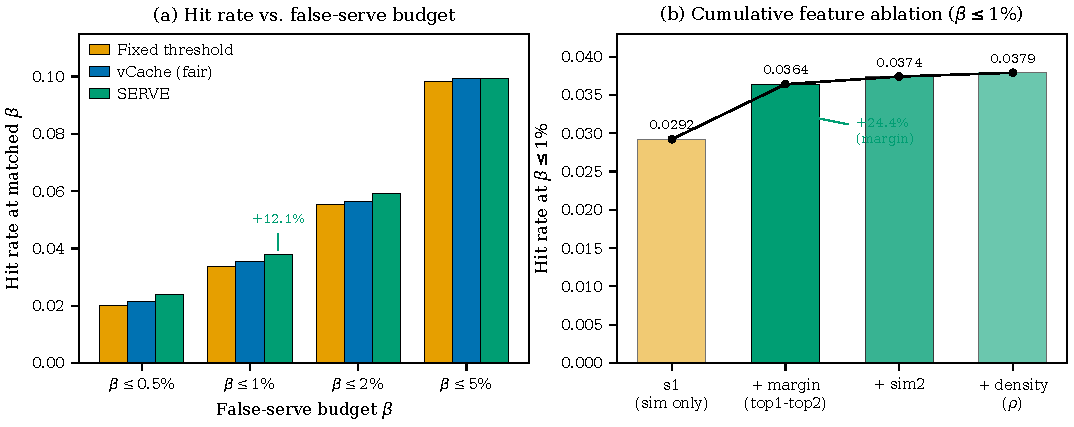
\includegraphics[width=\textwidth]{figures/fig1_sota_ablation.pdf}
\caption{\textbf{Left:} hit-rate at matched false-serve budget
(Table~\ref{tab:sota}) for the fixed threshold, the fair vCache
reimplementation, and SERVE, on 100k MiniLM QQP embeddings with a
60k-entry cache, 4 seeds. \textbf{Right:} one-feature-at-a-time ablation
at $\beta \le 1\%$, adding $s_1$, then $m$, then $s_2$, then $\rho$
(Eq.~\ref{eq:features}) in order; the margin term $m$ alone accounts for
the majority of SERVE's total improvement over a similarity-only gate.}
\label{fig:sota}
\end{figure*}

\subsection{Feature Ablation}

Table~\ref{tab:sota} establishes that the full feature vector
$\mathbf{x}$ (Eq.~\ref{eq:features}) beats both baselines. A skeptic could
grant that aggregate gain and still ask whether it is really the margin
doing the work, or four weak signals adding up to something not
mechanistically interpretable. We add features to
the gate one at a time, in order, and measure hit-rate at $\beta \le 1\%$
(Fig.~\ref{fig:sota}, right panel). Similarity alone ($\mathbf{x}=[s_1]$)
reaches 0.0292 -- close to, and consistent with, the fixed-threshold
baseline of 0.0338, since both are functions of $s_1$ under a monotone
decision rule. Adding the margin, $\mathbf{x}=[s_1, m]$
(Eq.~\ref{eq:margin}), raises hit-rate to 0.0364, a +24.4\% relative gain
over similarity alone. Adding the runner-up similarity $s_2$ on top of the
margin adds a further +3.0\% (to 0.0374), and adding local density $\rho$
(Eq.~\ref{eq:density}) on top of both adds a final +1.2\% (to 0.0379). The
margin term alone therefore recovers roughly 83\% of SERVE's total
improvement over a similarity-only gate ($\frac{0.0364-0.0292}{0.0379-0.0292} \approx 0.83$).
This is the central mechanistic finding of the paper: it is not that four
weak features combine into one strong gate; one specific, already-computed
quantity, the gap between the best match and the runner-up, is doing
almost all of the work that similarity alone cannot do, and it is exactly
the quantity both the fixed-threshold and vCache decision rules
(Eq.~\ref{eq:fixed}, \ref{eq:vcache}) discard by construction.

\subsection{Robustness to Embedding Quality}

A natural objection to the margin's advantage is that it might be an
artifact of ambiguity specific to a comparatively weak 384-dimensional
embedding, and would vanish with a stronger encoder that resolves the same
ambiguity on its own. We test this directly by rerunning the identical
protocol with a 768-dimensional mpnet checkpoint
\cite{song2020mpnet,reimers2019sentencebert}, comparing SERVE against the
fixed threshold only (Table~\ref{tab:embedding}, Fig.~\ref{fig:embedding}).
At $\beta \le 1\%$, the
relative gain narrows only modestly, from +11.6\% on MiniLM to +9.0\% on
mpnet, and does not come close to vanishing. This is consistent with the
margin capturing genuine ambiguity in the query population's decision
boundary -- cases where two candidate matches are both plausible -- rather
than compensating for embedding-specific noise that a stronger encoder
would otherwise resolve.

\begin{table}[t]
\centering
\caption{SERVE vs.\ fixed threshold at $\beta \le 1\%$ across embedding
checkpoints, 4 seeds each. mpnet run is stand-alone (no vCache
comparison in this experiment); its MiniLM row differs from
Table~\ref{tab:sota} by $<0.001$, within normal seed variation.}
\label{tab:embedding}
\begin{tabular}{lcccc}
\toprule
Embedding & Dim. & Fixed & SERVE & Rel.\ gain \\
\midrule
MiniLM \cite{wang2020minilm} & 384 & 0.0338 & 0.0377 & +11.6\% \\
mpnet \cite{song2020mpnet}   & 768 & 0.0351 & 0.0383 & +9.0\%  \\
\bottomrule
\end{tabular}
\end{table}

\begin{figure}[t]
\centering
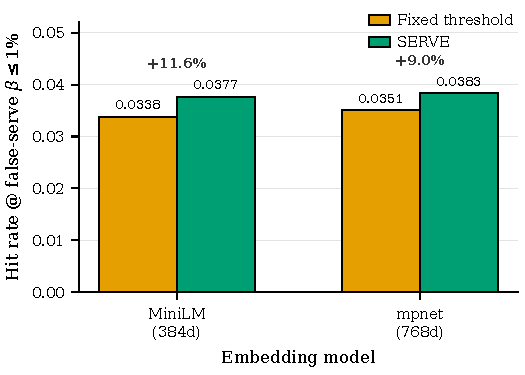
\includegraphics[width=\columnwidth]{figures/fig2_embedding_quality.pdf}
\caption{Hit-rate at $\beta \le 1\%$ for the fixed threshold versus SERVE
on MiniLM (384d) and mpnet (768d) embeddings, 4 seeds each
(Table~\ref{tab:embedding}). SERVE's relative advantage narrows only
modestly as embedding strength increases and remains large in both
settings.}
\label{fig:embedding}
\end{figure}

\subsection{Robustness to Query Recurrence}

If the margin's value came only from resolving rare edge cases in an
otherwise easy distribution, its contribution should shrink as recurrence
$r$ rises and the cache fills with genuine duplicates, since a denser true-match
pool should make $s_1$ alone more reliably decisive. We observe the
opposite: SERVE's relative gain over the fixed threshold at $\beta \le 1\%$
rises monotonically across the entire swept range of $r$
(Fig.~\ref{fig:recurrence}), from +20.9\% at $r=0.2$ to +77.8\% at
$r=0.9$. Higher recurrence does not make the decision easier; it increases
the fraction of traffic that consists of genuine near-duplicate collisions
sitting close to the decision boundary defined by~\eqref{eq:margin}, which
is precisely the regime the margin feature targets.

Crossing $r$ against $\beta$ in a joint $4\times3$ grid
(Table~\ref{tab:grid}, Fig.~\ref{fig:grid}) shows the two axes compound: relative gain rises
from +41.7\% at the loosest cell tested ($r=0.5$, $\beta \le 1\%$) to
+205.3\% at the strictest budget among the high-recurrence cells tested
($r=0.8$, $\beta \le 0.25\%$; fixed hit-rate 0.0231, SERVE hit-rate
0.0707). We report the full grid rather than isolating this single best
cell because the trend across both axes, not any one cell, is the
finding: the gain at $r=0.8$, $\beta \le 0.25\%$ is the grid maximum, at
or near the top of both the recurrence range and the strictness range
swept (note $r=0.9$ yields a nearly identical +205.2\% at the same
budget, so the two highest-recurrence cells are effectively tied),
meaning the benefit is driven jointly by high recurrence and a strict
false-serve budget, not either alone -- the combination commonly
associated with FAQ and customer-support caches, though we do not
directly measure production traffic to confirm that characterization
(\S\ref{sec:limitations}).

\begin{table}[t]
\centering
\caption{SERVE relative hit-rate gain over the fixed threshold (\%),
crossing query recurrence $r$ against false-serve budget $\beta$, 4 seeds
per cell.}
\label{tab:grid}
\begin{tabular}{lccc}
\toprule
$r$ & $\beta\le0.25\%$ & $\beta\le0.5\%$ & $\beta\le1\%$ \\
\midrule
0.5 & +154.4\% & +82.8\%  & +41.7\% \\
0.7 & +166.8\% & +120.3\% & +64.4\% \\
0.8 & \textbf{+205.3\%} & +141.9\% & +73.3\% \\
0.9 & +205.2\% & +140.1\% & +77.8\% \\
\bottomrule
\end{tabular}
\end{table}

\begin{figure}[t]
\centering
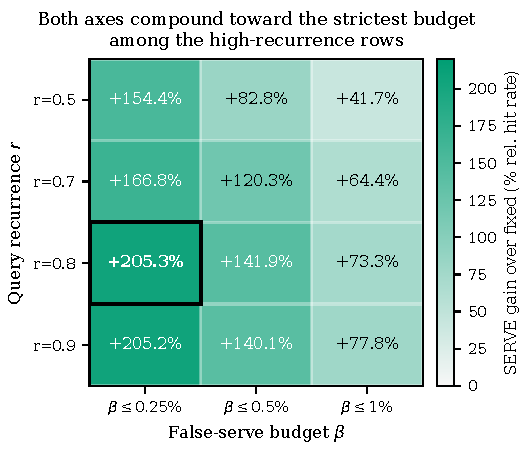
\includegraphics[width=\columnwidth]{figures/fig4_best_regime_grid.pdf}
\caption{Heatmap view of Table~\ref{tab:grid}: SERVE's relative hit-rate
gain over the fixed threshold (\%), crossing query recurrence $r$ against
false-serve budget $\beta$, 4 seeds per cell. Both axes push in the same
direction, and the gain is largest in the strictest-budget cell among the
high-recurrence rows (outlined).}
\label{fig:grid}
\end{figure}

\begin{figure}[t]
\centering
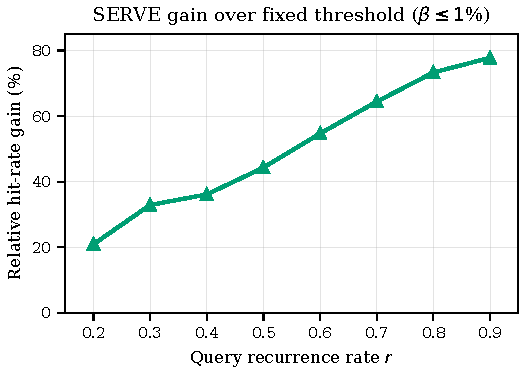
\includegraphics[width=\columnwidth]{figures/fig3_recurrence.pdf}
\caption{SERVE's relative hit-rate gain over the fixed threshold at
$\beta \le 1\%$, swept over query recurrence $r$ (fraction of test
queries with a genuine duplicate anywhere in the cache), 4 seeds per
point. Growth is monotonic across the full range $r \in [0.2, 0.9]$.}
\label{fig:recurrence}
\end{figure}

\subsection{External Validation on PAWS}

Every result above is measured on QQP with a cache/train/test split we
constructed ourselves. We rerun the identical protocol, unchanged, on PAWS
\cite{zhang2019paws}, an independently constructed benchmark whose
non-paraphrase pairs are built by word-scrambling a paraphrase pair,
producing exactly the high-lexical-overlap, ambiguous near-duplicate
regime~\eqref{eq:margin} targets, and not designed with SERVE in mind
(\S\ref{sec:setup}). The result is categorical rather than incremental
(Fig.~\ref{fig:paws}). The fixed-threshold baseline reaches AUC 0.1408 on
PAWS -- worse than the chance level of 0.5, i.e.\ actively
anti-correlated with the correct decision. This has a documented cause:
PAWS's word-scrambled non-paraphrases are systematically \emph{more}
cosine-similar than genuine same-meaning paraphrases, which is the reason
the benchmark was constructed, to break methods that cannot see past
shared surface vocabulary. A manually sign-corrected variant of the fixed
baseline (served on \emph{low} rather than high similarity, an unrealistic
correction that requires advance knowledge that the relationship is
inverted) recovers to AUC 0.8592. SERVE, trained the ordinary way with no
sign knowledge or manual correction, reaches AUC 0.9025 -- exceeding even
the hand-corrected, oracle-sign baseline by a further $+0.0433$ absolute.
The margin remains the dominant single feature on PAWS as well: at
$\beta \le 1\%$, similarity alone reaches hit-rate 0.0020, and adding the
margin alone raises it to 0.0044 (+118.8\% relative). On a benchmark not
built to favor this method, the naive deployed decision rule
(Eq.~\ref{eq:fixed}) is not merely suboptimal, it is wrong, and the
margin-aware gate is what makes the reuse decision usable at all in this
regime.

\begin{figure}[t]
\centering
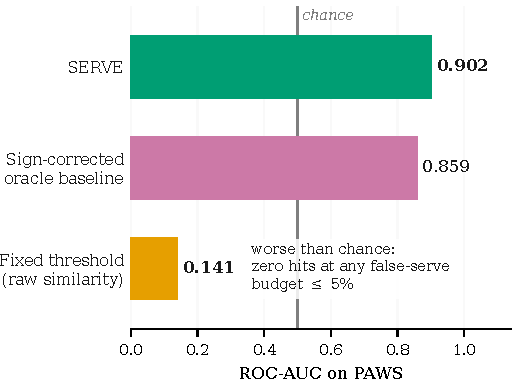
\includegraphics[width=\columnwidth]{figures/fig5_paws.pdf}
\caption{ROC-AUC on PAWS \cite{zhang2019paws} for the fixed
similarity-threshold baseline as published (0.1408, below the chance
line at 0.5), a manually sign-corrected oracle variant of the same
baseline (0.8592), and SERVE trained without any sign knowledge or
manual correction (0.9025). Train split (49{,}401 pairs) builds its own
cache and trains the gate; held-out test split (8{,}000 pairs) builds an
independent cache; zero sentence overlap verified between splits; same
MiniLM checkpoint as QQP.}
\label{fig:paws}
\end{figure}

\section{Discussion}
\label{sec:discussion}

The four features in $\mathbf{x}$ (Eq.~\ref{eq:features}) are all
byproducts of the top-$k$ nearest-neighbor search a semantic cache already
performs to find $s_1$; none require an additional embedding call or index
lookup relative to the fixed-threshold or vCache baselines. That makes the
practical implication direct: a cache operator running GPTCache-,
MeanCache-, or vCache-style reuse logic can compute $m$, $s_2$, and $\rho$
for free from data already in hand at decision time, and the results above
indicate doing so buys the largest improvement exactly under the two
conditions that define a production deployment -- a low tolerance for
false serves, and sustained repeat-query traffic (\S\ref{sec:results}D).

We also report a negative result from our own process, because it bears on
how much confidence to place in the positive result above. The feature we
initially expected to be the differentiator was not the margin but
cache-entry hubness -- a cache entry's nearest-neighbor in-degree over the
query population, motivated by the documented tendency of high-in-degree
points in high-dimensional nearest-neighbor search to become promiscuous,
hard-to-distinguish false matches \cite{radovanovic2010hubs}. We
implemented it as a fifth feature, added it to $\mathbf{x}$, and ablated it
under the identical protocol used for $s_1$, $m$, $s_2$, and $\rho$; its
effect on hit-rate at the matched false-serve budget was neutral to
slightly negative, so we dropped it and it is not part of the SERVE feature
set reported here. We view this as evidence of, not a distraction from,
the rigor of the positive result: the same ablation discipline that
identified the margin as the dominant feature also killed our own
initially preferred hypothesis when the evidence did not support it.

Finally, we did not test this directly, so we state it only as a
plausible extension, not a result: the margin between a top match and its
runner-up is a general byproduct of any nearest-neighbor search, not a
property specific to semantic caching, which raises the possibility that
other systems that make a keep-or-reject decision from a top-1 retrieval
(e.g.\ deduplication or retrieval-augmented generation gating) discard the
same signal by construction. Whether the same gain materializes there is a
question this study does not test.

\section{Limitations}
\label{sec:limitations}

Results are reported on two datasets (QQP, PAWS) and two embedding models
(MiniLM, mpnet); a broader sweep of embedding families and domains (code
search, multilingual, retrieval-augmented-generation corpora) was not run,
and we make no claim that the margin's advantage transfers unchanged to
those settings, only that it holds across the two axes tested. SERVE is a
small gradient-boosted model retrained per cache configuration rather than
one that updates online as a cache's content drifts; how the gate should be
refreshed in a live, drifting deployment was not studied. The comparison to
vCache uses a fair reimplementation of its published per-embedding
calibrated-threshold mechanism (Eq.~\ref{eq:vcache}) rather than the
original vCache codebase, and we report that choice plainly rather than
presenting it as equivalent to the original system. The high-recurrence
regime we describe as characteristic of FAQ and customer-support caches
(\S\ref{sec:results}D) is constructed by direct manipulation of $r$ in the
test-query population, not measured from real production traffic.

\section{Conclusion}

Two deployed decision rules for semantic-cache reuse, a fixed
cosine-similarity threshold and vCache's per-embedding calibrated
threshold, both reduce the decision to a function of $s_1$ alone. A
gradient-boosted gate over the retrieval geometry they discard, with the
margin term as the dominant contributor, improves cache hit-rate at a
matched false-serve budget over both baselines on real QQP data, holds up
on a stronger embedding, grows rather than shrinks under realistic repeat-
query traffic, and turns an actively wrong baseline into a strongly
discriminative one on an external adversarial benchmark it was not designed
to favor. The gain is small when averaged over all operating points, but it
is largest in the low-false-serve, high-recurrence regime that production
caches are actually run in.

\bibliographystyle{IEEEtran}
\bibliography{refs}

\end{document}
